\chapter{Results and Discussion}
For the test of the algorithm different scenarios have been chosen and simulations were conducted to test the efficiency and accuracy of the path planning. The scenarios chosen for the simulation describe common problems path planning algorithms need to be able to overcome in order to be usable for the navigation in unstructured environments. The first problem The problems are depicted in \Fref{fig:scenarioDeadEnd}, \Fref{fig:scenarioParkingStructure} and \Fref{fig:scenarioRandomObstacles}.

The scenarios shall test the algorithm for different scenarios.

\begin{figure}[h]
    \includegraphicsTex{scenarioDeadEnd.pdf_tex}
    \caption{The dead end scenario}
    \label{fig:scenarioDeadEnd}
\end{figure}

\begin{figure}[h]
    \includegraphicsTex{scenarioParkingStructure.pdf_tex}
    \caption{The parking structure scenario}
    \label{fig:scenarioParkingStructure}
\end{figure}

\begin{figure}[h]
    \includegraphicsTex{scenarioRandomObstacles.pdf_tex}
    \caption{The random obstacles scenario}
    \label{fig:scenarioRandomObstacles}
\end{figure}

\section{Results}

\subsection{Simulation Results}

\begin{figure}[h]
    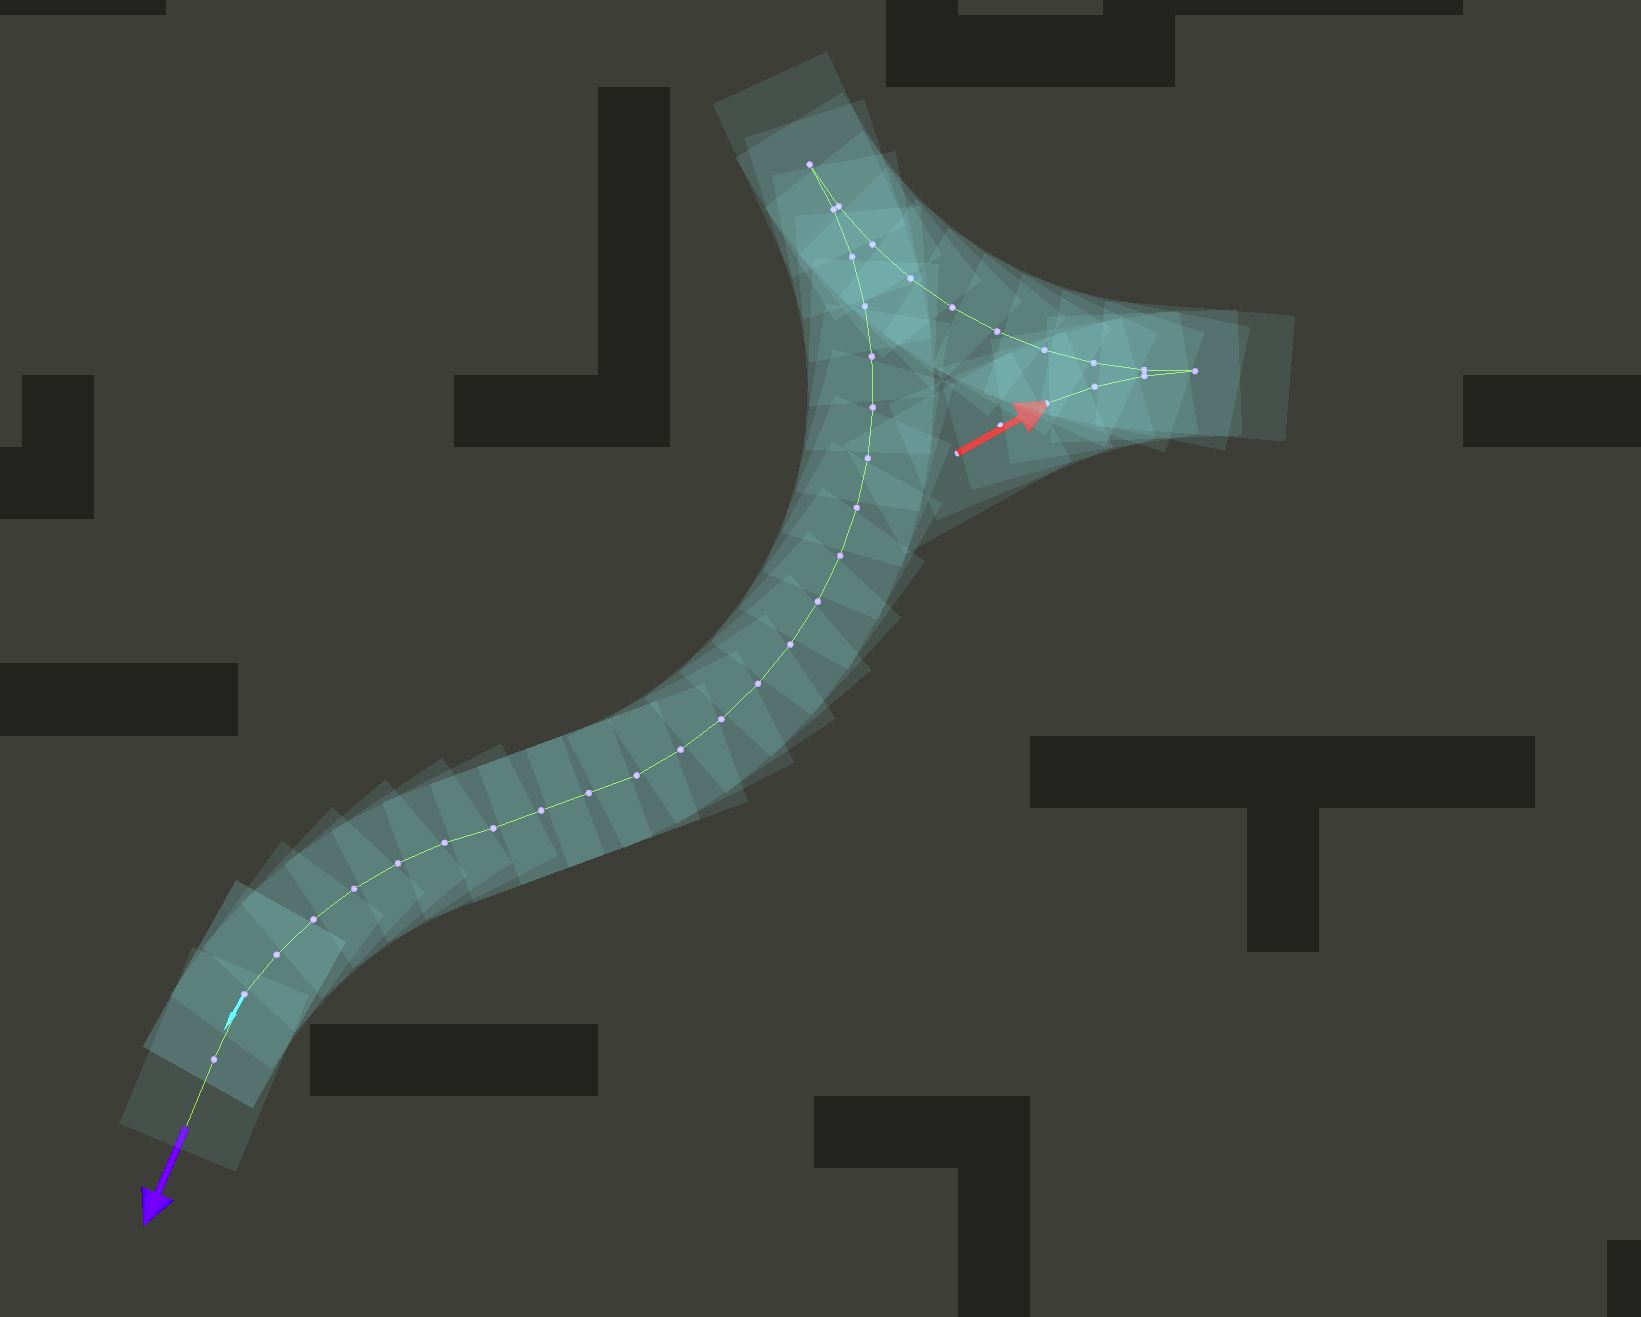
\includegraphics[width=\textwidth]{threePointTurn.png}
    \caption{Three point turn for change of directions}
    \label{fig:threePointTurn}
\end{figure}

\begin{figure}[h]
    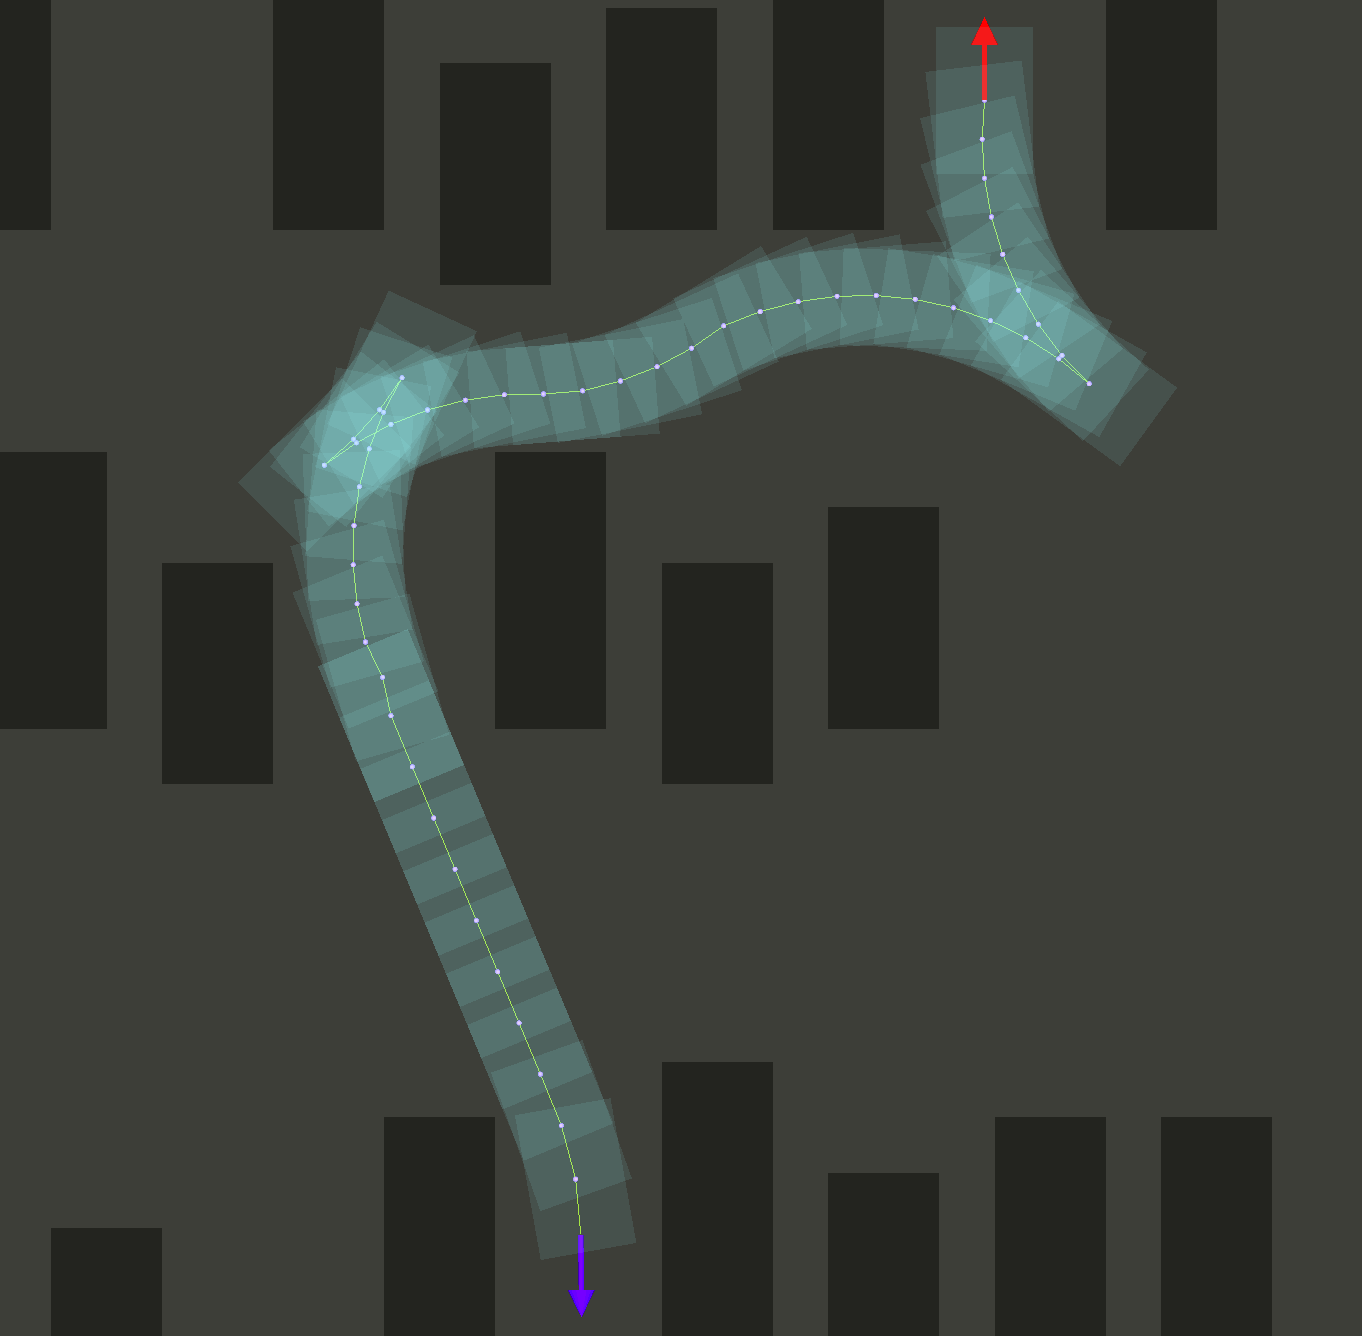
\includegraphics[width=\textwidth]{parking.png}
    \caption{Change of parking spot in a parking lot}
    \label{fig:parking}
\end{figure}

\subsection{Real-world Results}

\section{Analysis}